
    \documentclass[border=10pt, 12pt]{standalone}
    \usepackage[svgnames]{xcolor}
    \usepackage{amsmath}
    \usepackage{pgfplots}
    \pgfplotsset{compat=newest}
    \usepackage[sfdefault]{FiraSans}
    \usepackage{FiraMono}
    \renewcommand*\familydefault{\sfdefault}
    \begin{document}
    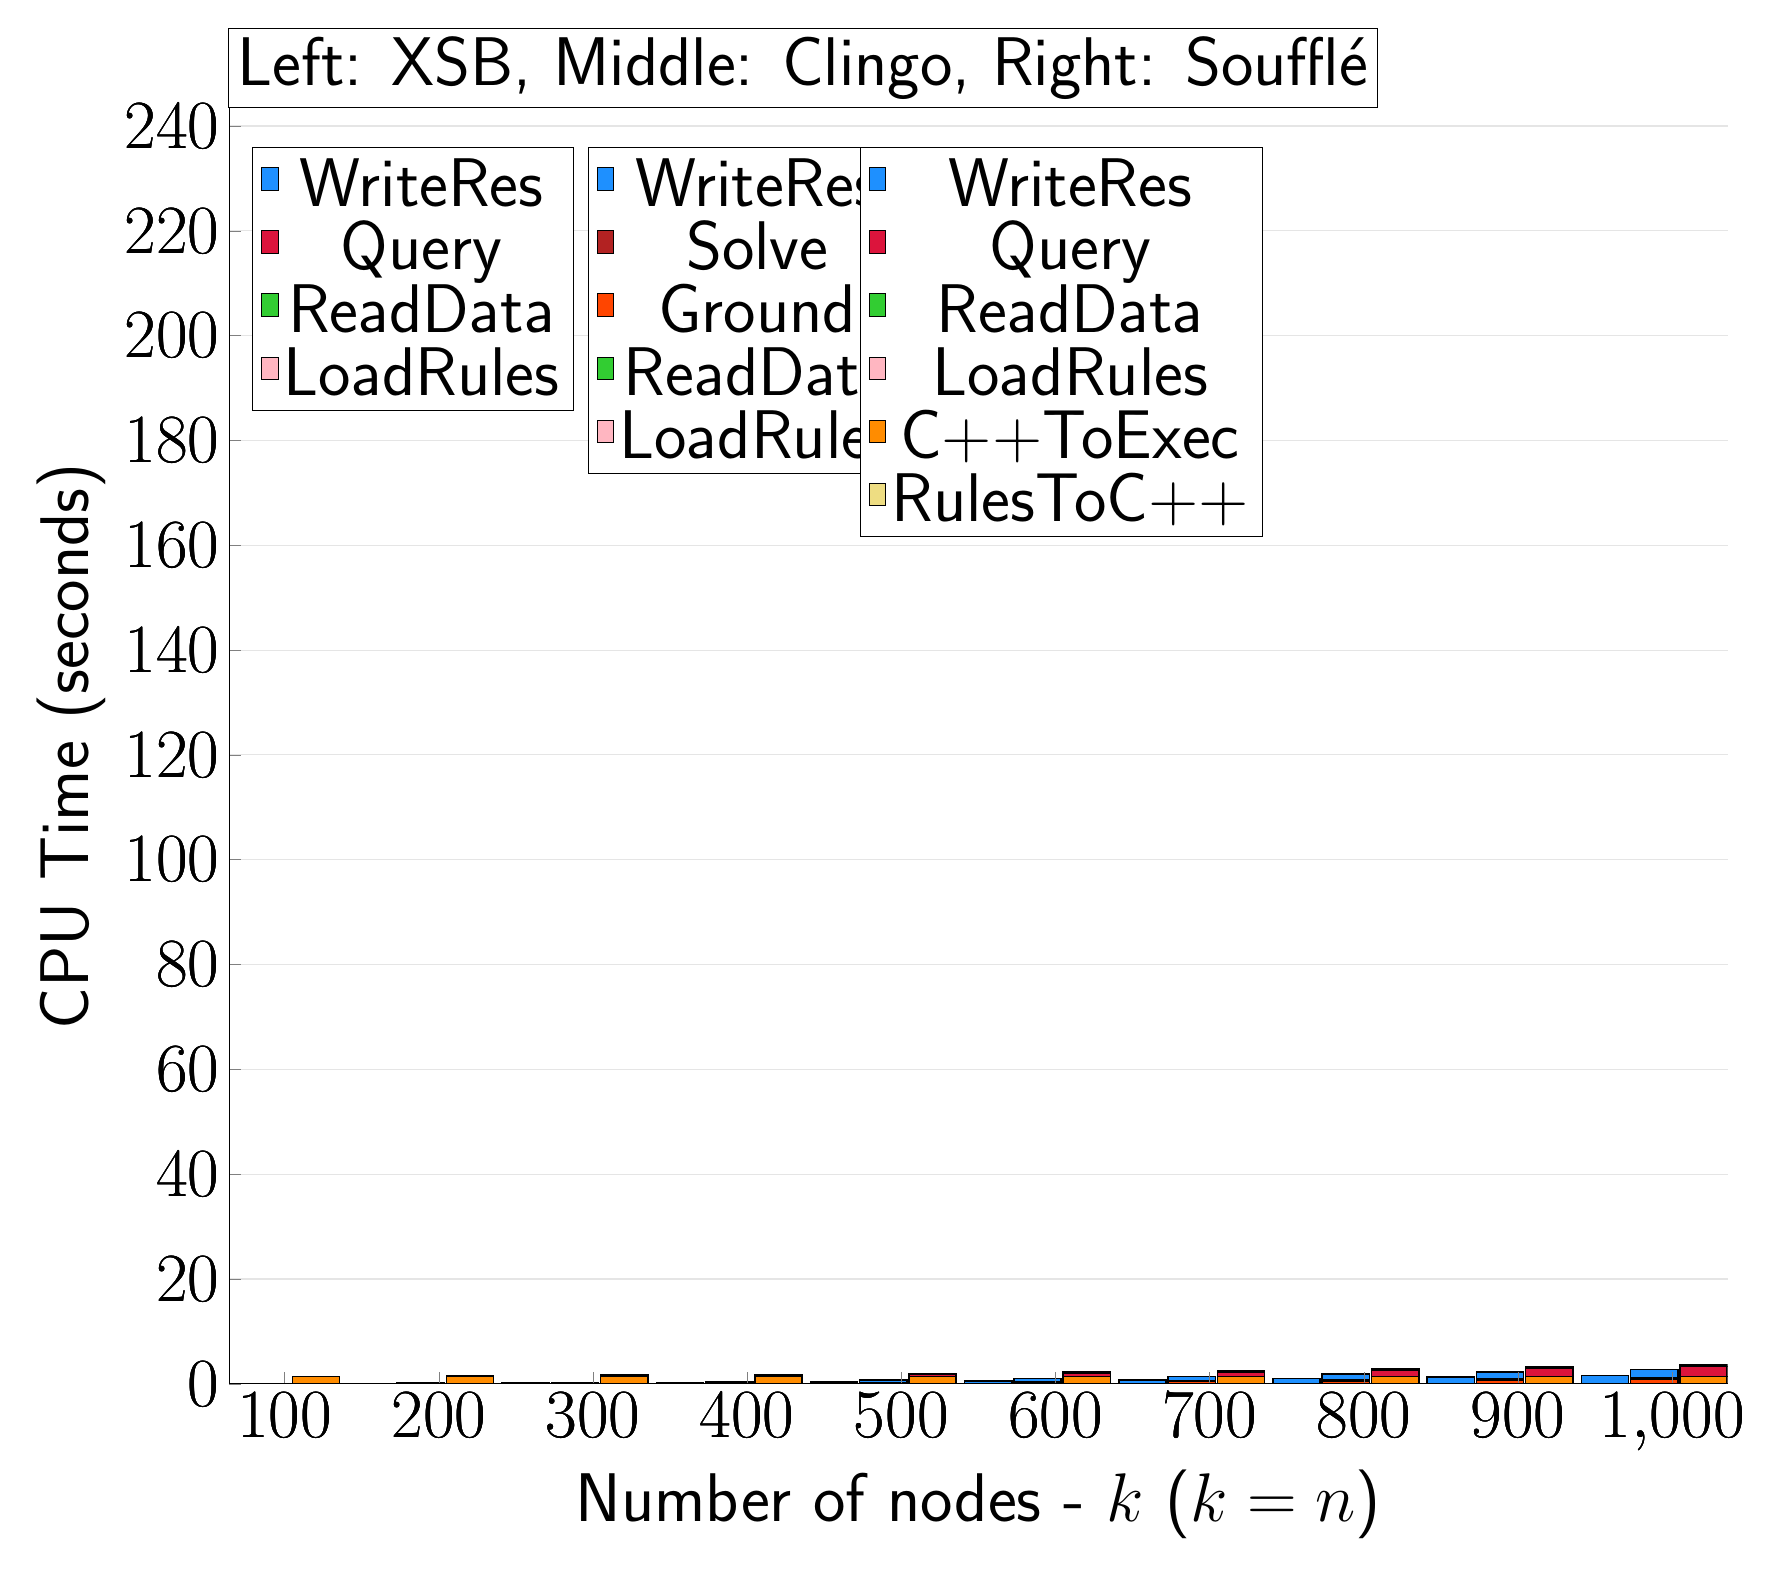
\begin{tikzpicture}
                            \begin{axis}[bar shift=-24.3pt, 
   ybar stacked,
   width=1.7\textwidth,
   bar width=0.6cm,
   ymajorgrids, tick align=inside,
   major grid style={draw=gray!20},
   xtick=data,
   ymin=0, ymax=243.3584,
   axis x line*=bottom,
   axis y line*=left,
   enlarge x limits=0.04,
   legend style={
       at={(0.23, 0.97)},
       anchor=north east,
       legend columns=1,
       font=\Huge,
   },
   ylabel={CPU Time (seconds)},
   xlabel={Number of nodes - $k$ ($k=n$)},
   label style={font=\Huge},
   tick label style={font=\Huge},
]
\addlegendimage{fill=DodgerBlue, draw=black, line width=0.2pt}
\addlegendentry{WriteRes}
\addlegendimage{fill=Crimson, draw=black, line width=0.2pt}
\addlegendentry{Query}
\addlegendimage{fill=LimeGreen, draw=black, line width=0.2pt}
\addlegendentry{ReadData}
\addlegendimage{fill=LightPink, draw=black, line width=0.2pt}
\addlegendentry{LoadRules}
\addplot +[fill=LightPink, draw=black, line width=0.55pt] coordinates {
(100, 0.0006279999999999998)
(200, 0.0006136000000000002)
(300, 0.0006087999999999993)
(400, 0.0006103999999999988)
(500, 0.0006103999999999994)
(600, 0.0006005999999999995)
(700, 0.0006150000000000002)
(800, 0.0006208000000000011)
(900, 0.0006202000000000002)
(1000, 0.0006190000000000012)
};
\addplot +[fill=LimeGreen, draw=black, line width=0.55pt] coordinates {
(100, 0.0002916000000000008)
(200, 0.00046779999999999966)
(300, 0.000621200000000001)
(400, 0.0007944000000000007)
(500, 0.0009472000000000001)
(600, 0.0011136)
(700, 0.0013204)
(800, 0.0014772000000000001)
(900, 0.0016805999999999998)
(1000, 0.0018368000000000002)
};
\addplot +[fill=Crimson, draw=black, line width=0.55pt] coordinates {
(100, 0.000926599999999999)
(200, 0.0035356)
(300, 0.0078334)
(400, 0.0140086)
(500, 0.0217034)
(600, 0.0313932)
(700, 0.0427108)
(800, 0.0556354)
(900, 0.0710152)
(1000, 0.0874314)
};
\addplot +[fill=DodgerBlue, draw=black, line width=0.55pt] coordinates {
(100, 0.015223400000000002)
(200, 0.06269079999999999)
(300, 0.13369780000000003)
(400, 0.23917259999999999)
(500, 0.37012480000000003)
(600, 0.5385302)
(700, 0.7295326)
(800, 0.9591581999999998)
(900, 1.2041574)
(1000, 1.4923116)
};
\end{axis}

\begin{axis}[bar shift=-6.5pt, 
   ybar stacked,
   width=1.7\textwidth,
   bar width=0.6cm,
   ymajorgrids, tick align=inside,
   major grid style={draw=none},
   xtick=data,
   ymin=0, ymax=243.3584,
   axis x line*=none,
   axis y line*=none,
   enlarge x limits=0.04,
   legend style={
       at={(0.454, 0.97)},
       anchor=north east,
       legend columns=1,
       font=\Huge,
   },
   label style={font=\Huge},
   tick label style={font=\Huge},
]
\addlegendimage{fill=DodgerBlue, draw=black, line width=0.2pt}
\addlegendentry{WriteRes}
\addlegendimage{fill=FireBrick, draw=black, line width=0.2pt}
\addlegendentry{Solve}
\addlegendimage{fill=OrangeRed, draw=black, line width=0.2pt}
\addlegendentry{Ground}
\addlegendimage{fill=LimeGreen, draw=black, line width=0.2pt}
\addlegendentry{ReadData}
\addlegendimage{fill=LightPink, draw=black, line width=0.2pt}
\addlegendentry{LoadRules}
\addplot +[fill=LightPink, draw=black, line width=0.55pt] coordinates {
(100, 0.0)
(200, 0.0)
(300, 0.0)
(400, 0.0)
(500, 0.0)
(600, 0.0)
(700, 0.0)
(800, 0.0)
(900, 0.0)
(1000, 0.0)
};
\addplot +[fill=LimeGreen, draw=black, line width=0.55pt] coordinates {
(100, 0.0020000000000000018)
(200, 0.0)
(300, 0.0)
(400, 0.0)
(500, 0.0)
(600, 0.0019999999999999905)
(700, 0.005999999999999983)
(800, 0.0020000000000000018)
(900, 0.004000000000000001)
(1000, 0.010000000000000009)
};
\addplot +[fill=OrangeRed, draw=black, line width=0.55pt] coordinates {
(100, 0.007999999999999997)
(200, 0.03400000000000001)
(300, 0.07399999999999998)
(400, 0.12600000000000006)
(500, 0.20600000000000002)
(600, 0.316)
(700, 0.43)
(800, 0.5860000000000001)
(900, 0.722)
(1000, 0.8879999999999999)
};
\addplot +[fill=FireBrick, draw=black, line width=0.55pt] coordinates {
(100, 0.0)
(200, 0.006000000000000005)
(300, 0.014000000000000012)
(400, 0.030000000000000027)
(500, 0.04200000000000004)
(600, 0.06000000000000005)
(700, 0.08400000000000007)
(800, 0.1080000000000001)
(900, 0.15599999999999992)
(1000, 0.18199999999999994)
};
\addplot +[fill=DodgerBlue, draw=black, line width=0.55pt] coordinates {
(100, 0.020000000000000018)
(200, 0.07)
(300, 0.16200000000000003)
(400, 0.2719999999999999)
(500, 0.43199999999999994)
(600, 0.6259999999999999)
(700, 0.8639999999999999)
(800, 1.1439999999999997)
(900, 1.366)
(1000, 1.688)
};
\end{axis}

\begin{axis}[bar shift=11.3pt, 
   ybar stacked,
   width=1.7\textwidth,
   bar width=0.6cm,
   ymajorgrids, tick align=inside,
   major grid style={draw=none},
   xtick=data,
   ymin=0, ymax=243.3584,
   axis x line*=none,
   axis y line*=none,
   enlarge x limits=0.04,
   legend style={
       at={(0.69, 0.97)},
       anchor=north east,
       legend columns=1,
       font=\Huge,
   },
   label style={font=\Huge},
   tick label style={font=\Huge},
]
\addlegendimage{fill=DodgerBlue, draw=black, line width=0.2pt}
\addlegendentry{WriteRes}
\addlegendimage{fill=Crimson, draw=black, line width=0.2pt}
\addlegendentry{Query}
\addlegendimage{fill=LimeGreen, draw=black, line width=0.2pt}
\addlegendentry{ReadData}
\addlegendimage{fill=LightPink, draw=black, line width=0.2pt}
\addlegendentry{LoadRules}
\addlegendimage{fill=DarkOrange, draw=black, line width=0.2pt}
\addlegendentry{C++ToExec}
\addlegendimage{fill=LightGoldenrod, draw=black, line width=0.2pt}
\addlegendentry{RulesToC++}
\addplot +[fill=LightGoldenrod, draw=black, line width=0.55pt] coordinates {
(100, 0.006)
(200, 0.006000000000000003)
(300, 0.006000000000000005)
(400, 0.003999999999999998)
(500, 0.007999999999999997)
(600, 0.009999999999999998)
(700, 0.003999999999999998)
(800, 0.003999999999999998)
(900, 0.006)
(1000, 0.005999999999999997)
};
\addplot +[fill=DarkOrange, draw=black, line width=0.55pt] coordinates {
(100, 1.3940000000000001)
(200, 1.4620000000000002)
(300, 1.4360000000000002)
(400, 1.3800000000000001)
(500, 1.392)
(600, 1.4140000000000001)
(700, 1.3960000000000004)
(800, 1.4000000000000004)
(900, 1.372)
(1000, 1.372)
};
\addplot +[fill=LightPink, draw=black, line width=0.55pt] coordinates {
(100, 0.000113)
(200, 0.000156)
(300, 0.0001644)
(400, 0.0001536)
(500, 0.0001406)
(600, 0.0001434)
(700, 0.000115)
(800, 0.0001082)
(900, 0.00014819999999999997)
(1000, 0.00014099999999999998)
};
\addplot +[fill=LimeGreen, draw=black, line width=0.55pt] coordinates {
(100, 0.0007693999999999999)
(200, 0.0015172000000000002)
(300, 0.0016534)
(400, 0.0023740000000000002)
(500, 0.0030864000000000004)
(600, 0.0035223999999999997)
(700, 0.0035202000000000002)
(800, 0.0041605999999999995)
(900, 0.005353200000000001)
(1000, 0.0051354)
};
\addplot +[fill=Crimson, draw=black, line width=0.55pt] coordinates {
(100, 0.0240936)
(200, 0.08407300000000001)
(300, 0.1700792)
(400, 0.2912916)
(500, 0.45283860000000004)
(600, 0.6859024)
(700, 0.9016770000000001)
(800, 1.194874)
(900, 1.5825939999999998)
(1000, 1.889606)
};
\addplot +[fill=DodgerBlue, draw=black, line width=0.55pt] coordinates {
(100, 0.0044608)
(200, 0.012864800000000001)
(300, 0.028742800000000002)
(400, 0.0509436)
(500, 0.077478)
(600, 0.11246099999999999)
(700, 0.1545972)
(800, 0.1997032)
(900, 0.2561948)
(1000, 0.31440619999999997)
};
\end{axis}


    \node[anchor=south, draw, fill=white] at (rel axis cs:0.42, 1) {\Huge Left: XSB, Middle: Clingo, Right: Soufflé};
    \end{tikzpicture}
    \end{document}
                        